 \documentclass{beamer}

%\usecolortheme[RGB={170,130,220}]{structure}
\setbeamertemplate{items}[ball]
\setbeamertemplate{blocks}[rounded][shadow=true]
%\beamertemplateshadingbackground{yellow!15}{magenta!15}
\usetheme{Singapore}

\usepackage{amsmath, amsthm, amssymb, enumerate, natbib}
\usepackage{graphicx, epsfig}
\usepackage{setspace}
\usepackage{color}

\definecolor{darkgreen}{rgb}{0,0.4,0}
\definecolor{cgreen}{rgb}{0,0.5,0}
\definecolor{darkblue}{rgb}{0,0,0.6}
\definecolor{darkred}{rgb}{0.7,0,0.1}
\definecolor{lessdarkgreen}{rgb}{0.2,0.5,0}
\definecolor{darkerred}{rgb}{0.5,0.1,0.05}
\definecolor{lessdarkred}{rgb}{0.8,0,0}
\definecolor{purple}{rgb}{0.8,.0,0.9}
\definecolor{darkpurple}{rgb}{0.45,.0,1.0}
\definecolor{darkerpurple}{rgb}{0.5,.2,.9}
\definecolor{brightred}{rgb}{1,0,0}


\mode<presentation> {
  \usetheme{Singapore}
  % or ...

  \setbeamercovered{transparent}
  % or whatever (possibly just delete it)
}

\usepackage[english]{babel}
\usepackage[latin1]{inputenc}
\usepackage{times}
\usepackage[T1]{fontenc}
\usepackage{framed}

\newtheorem{proposition}[theorem]{Proposition}
\theoremstyle{definition}
\newtheorem{remark}[theorem]{Remark}
\newtheorem{algorithm}[theorem]{Algorithm}

\begin{document}


\title{\textbf{\LARGE{flowReMix}}  \\ (temporary name)  \vspace{ 1 cm }\\ \large{A \textbf{Mixture} of \textbf{Mixed} Beta-Binomial \textbf{Regression} Models for Analyzing \textbf{Flow}-Cytometry Count data}}

\vspace{1 cm}

%%%%%%%%%%%%%%%%%%%%%%%%%%%%%%%%%%%%%%%%%

\begin{frame}[plain]
  \titlepage
\end{frame}


%%%%%%%%%%%%%%%%%%%%%%%%%%%%%%%%%%%%%%%%%%%%%%%

\begin{frame}
\frametitle{Outline}
\begin{enumerate}
\item Introduction to Flow-Cytometry
\vspace{0.3 cm}
\item Motivation
\vspace{0.3 cm}
\item Models:
	\begin{itemize}
	\item A Marginal Model
	\item A Joint HMRF model
	\end{itemize}
	\vspace{0.3 cm}
\item Data analysis. 

\vspace{0.3 cm}
\item  Computation
\end{enumerate}
\end{frame}

%%%%%%%%%%%%%%%%%%%%%%%%%%%%%%%%%%%%%%%

\begin{frame}
\frametitle{Introduction to Cytometry Count Data}
\begin{center}
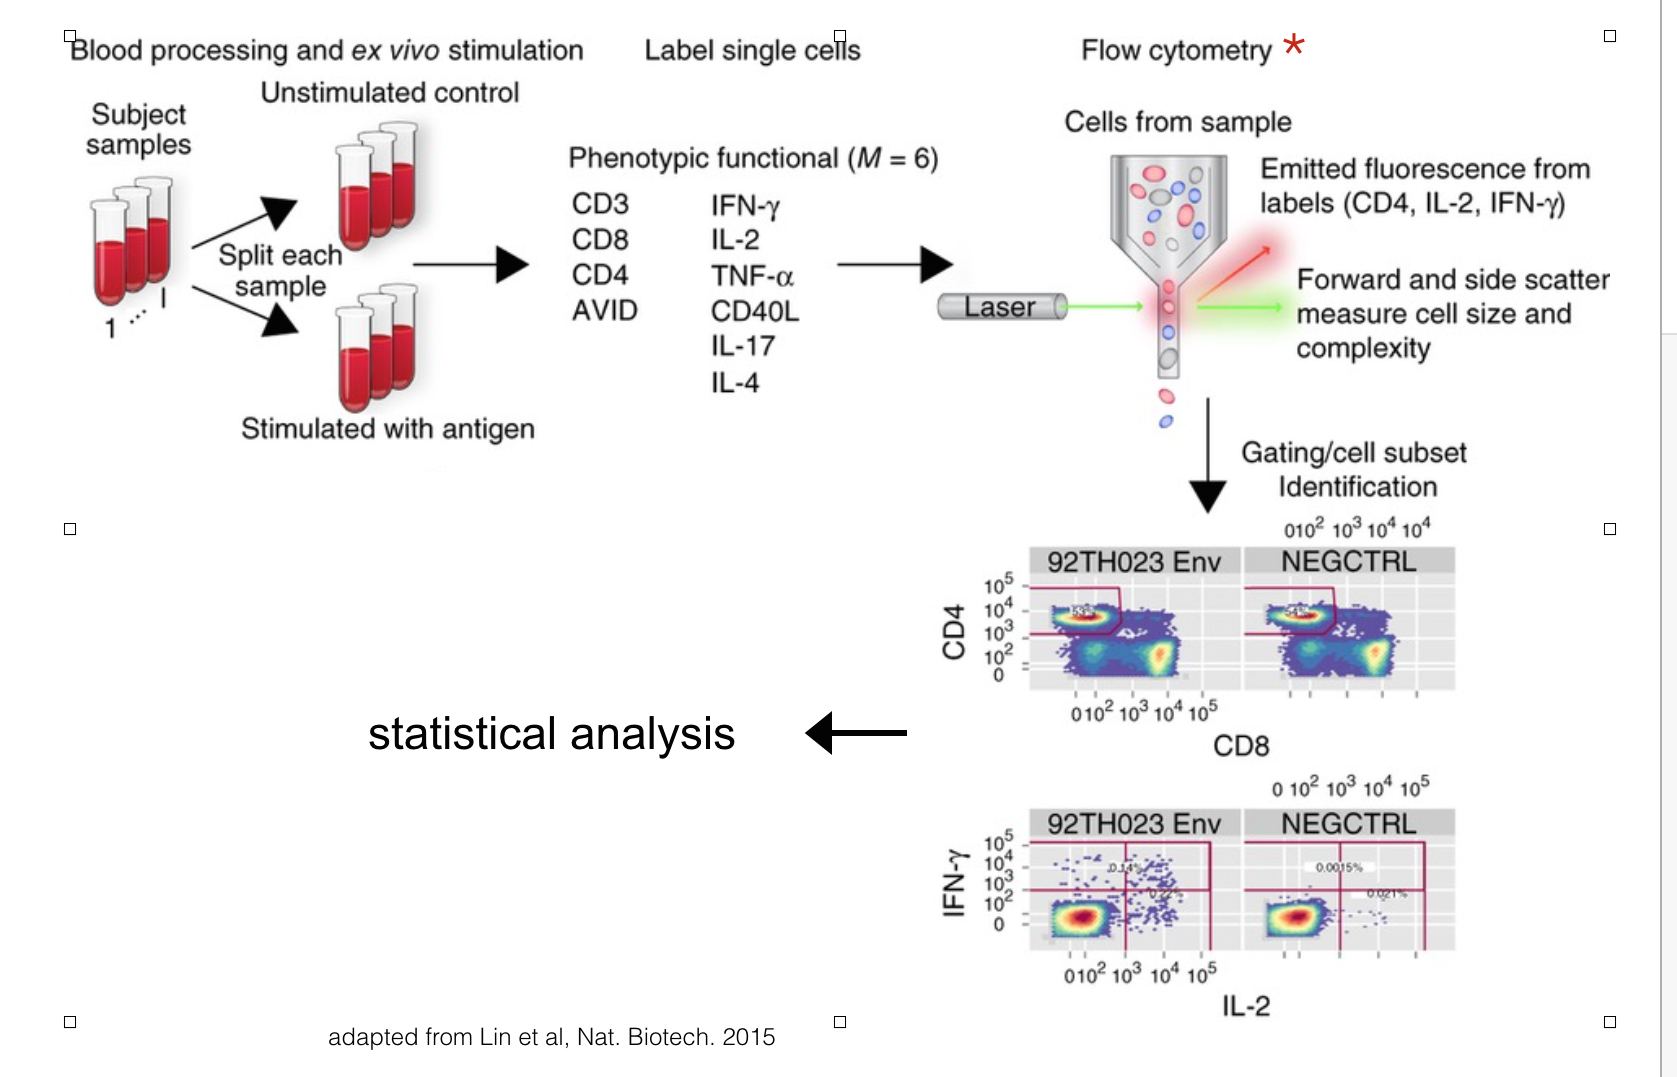
\includegraphics[scale=0.4]{figures/flowcytintro}
\end{center}
\end{frame}


%%%%%%%%%%%%%%%%%%%%%%%%%%%%%%%%%%%%%%%%%%%%%%%

\begin{frame}
\frametitle{Introduction to Cytometry Count Data}
\begin{figure}[]
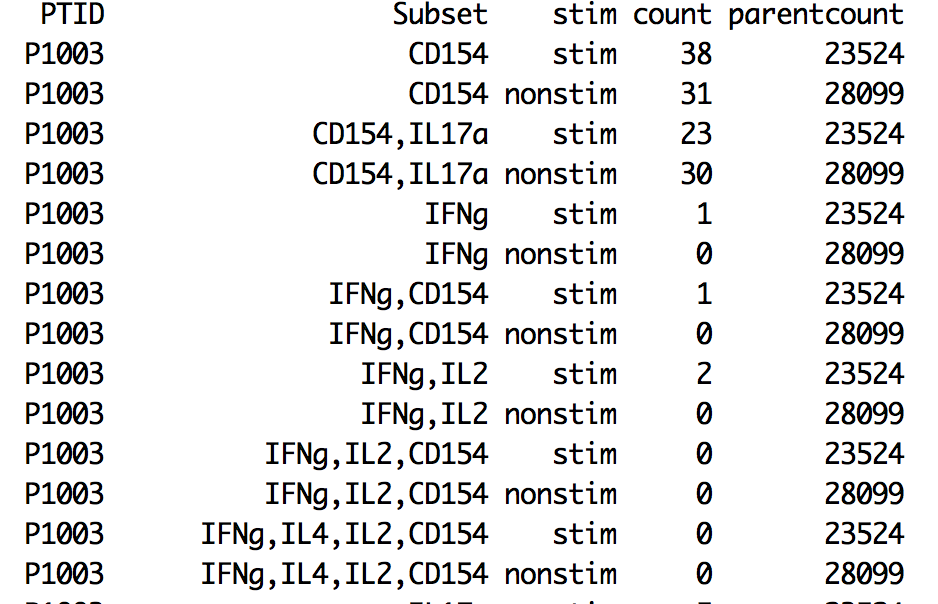
\includegraphics[width=12 cm]{figures/datasetExample} \caption{}
\end{figure}
\end{frame}

%%%%%%%%%%%%%%%%%%%%%%%%%%%%%%%%%%%%%%%%%%%%%%%

\begin{frame}
\frametitle{The RV144 HIV Vaccine Study}
\begin{itemize}
\item \textbf{286 Subjects}
	\begin{itemize}
	\item 246 Cases
	\item 40 Controls
	\end{itemize}
\vspace{0.2 cm}
\item \textbf{2 Types of stimulus} 
	\begin{itemize}
	\item HIV antigen
	\item Negative control
	\end{itemize}
\vspace{0.2 cm}
\item \textbf{6 types of cytokines.} 
\end{itemize}
\end{frame}

%%%%%%%%%%%%%%%%%%%%%%%%%%%%%%%%%%%%%%%%

\begin{frame}
\frametitle{Marginal Counts for RV144}
\begin{center}
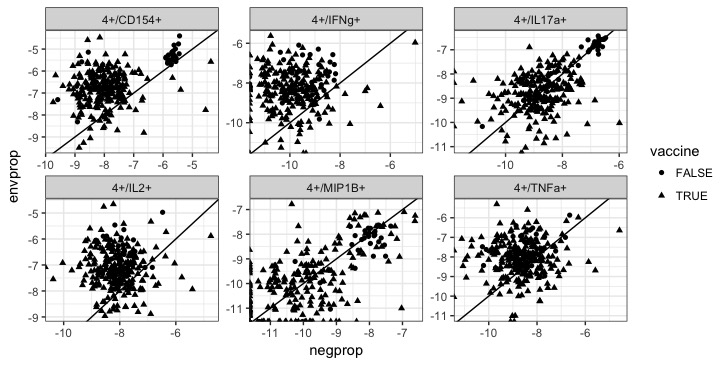
\includegraphics[scale=0.4]{figures/marginalScatterNoPost}
\end{center}
\end{frame}

%%%%%%%%%%%%%%%%%%%%%%%%%%%%%%%%%%%%%%%%

\begin{frame}
\frametitle{Motivation: COMPASS}
\begin{center}

\includegraphics[scale=0.18]{figures/compassCaption}
\end{center}

\pause
\textbf{Or in general, with immune response.}
\end{frame}

%%%%%%%%%%%%%%%%%%%%%%%%%%%%%%%%%%%%%%%%

\begin{frame}
\frametitle{How do current methods work? (Approximately)}
Current models are baseline/stimulation models. 
\begin{itemize}
\item  Unstimulated blood sample are compared stimulated ones.
\end{itemize}
\vspace{0.3 cm}

\pause
For the unstimulated sample of the $i$th subject out of $n$, we sample a count proportion:
$$
p_{i0} \sim \text{Dirichlet}(\alpha_{0},\beta_{0}),
$$$$
y_{i0} \sim \text{Multinomial}(N_{i0}, p_{i0}).
$$


\vspace{0.3 cm}
\pause
Let $k_i \in \{0,1\}^{p}$ indicate in which subsets $i$ responds:
$$
k_{ij} \sim \text{Ber}(w_j),
$$$$
p_{i1,\tau = 0} \sim \delta(p_{i0,\tau = 0}), \;\;\;\;
p_{i1, \tau = 1} | p_{i0,\tau = 0}  \propto \text{Dirichlet}(\alpha_1, \beta_{1})
$$$$
y_{i1} \sim \text{Multinomial}(N_{i1}, p_{i1})
$$
\end{frame}

%%%%%%%%%%%%%%%%%%%%%%%%%%%%%%%%%%%%%%%%%%%%%%%

\begin{frame}
\frametitle{Controlled Human Malaria Infection Study}
\begin{itemize}
\item 9 Tanzanian adults were infected with Malaria.
	\begin{itemize}
	\item +3 controls.
	\end{itemize}
	\vspace{0.75 cm}
	
\item Blood samples were collected at 6 time points.
	\begin{itemize}
	\item Day 0, day 9, blood  parasitemia, Day 28, Day 56, Day 168.
	\end{itemize}
	\vspace{0.75 cm}

\item Two types of stimulation:
	\begin{itemize}
	\item Infected/uninfected blood-cells.
	\end{itemize}
	\vspace{0.75 cm}
	
\item 113 measured cell-types divided into 8 groups. 
\end{itemize}
\end{frame}

%%%%%%%%%%%%%%%%%%%%%%%%%%%%%%%%%%%%%%%%

\begin{frame}
\frametitle{Controlled Human Malaria Infection Study}
\begin{center}
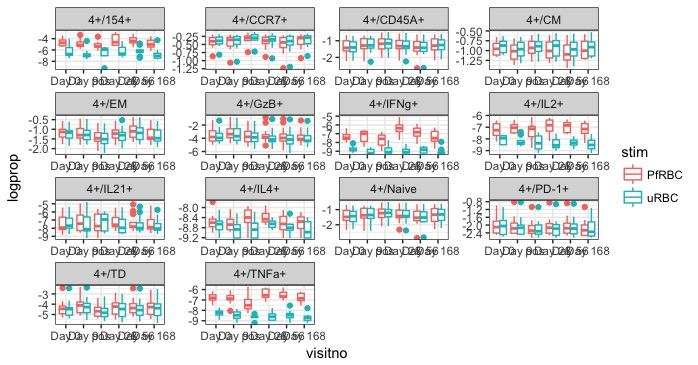
\includegraphics[scale=0.475]{figures/CHMIboxplot}
\end{center}
\end{frame}

%%%%%%%%%%%%%%%%%%%%%%%%%%%%%%%%%%%%%%%%

\begin{frame}
\frametitle{Motivation - A Regression Model}
\begin{itemize}
\item We want to be able to include covariates:
	\begin{itemize}
	\item Batch effects.
	\item Other covariates such as age, gender...
	\end{itemize}

\pause
\vspace{0.7 cm}
\item Longitudal data.

\vspace{0.7 cm}
\item More than one stimulation.

\pause
\vspace{0.7 cm}
\item Explicit dependence model:
	\begin{itemize}
	\item For the observed proportions.
	\item For response/non-response.
	\end{itemize}
\end{itemize}
\end{frame}

%%%%%%%%%%%%%%%%%%%%%%%%%%%%%%%%%%%%%%%%%%%%%%%

\begin{frame}
\frametitle{Motivation - Unique Challanges}
\begin{itemize}
\item \textbf{Dependence}
	\begin{itemize}
	\item Within sample between cell subsets.
	\item Within subject / across time.  
	\end{itemize}
\vspace{0.76 cm}
\item \textbf{Heterogenous treatment effect}
\vspace{0.76 cm}
\item \textbf{Over-dispersed Binomial counts}
\end{itemize}
\end{frame}

%%%%%%%%%%%%%%%%%%%%%%%%%%%%%%%%%%%%%%%%%%%%%%%

\begin{frame}
\frametitle{A Marginal Model - Single Subset}
\begin{framed}
Indexing: \textbf{i}-subject, \textbf{t}- stimulation/time-point.
\end{framed}

\begin{itemize}
\item Binomial count data $\Rightarrow$ Logistic model.
$$
\text{logit}(p_{it}) = X_{it} \beta
$$$$
y_{it} \sim \text{Binom}(N_{it}, p_{it})
$$

\pause
\item Dependence $\Rightarrow$ `random' subject baseline:
$$
\text{logit}(p_{it}) = X_{it} \beta + \nu_i
$$$$
\nu_i \sim N(0, \sigma^{2})
$$
\end{itemize}
\end{frame}

%%%%%%%%%%%%%%%%%%%%%%%%%%%%%%%%%%%%%%%%%%%%%%%]

\begin{frame}
\frametitle{A Marginal Model - Single Subset}
\begin{framed}
Indexing: \textbf{i}-subject, \textbf{t}- stimulation, \textbf{k}- cluster.
\end{framed}

\begin{itemize}
\item Non-response $\Rightarrow$ Mixture-Model:
$$
\text{logit}(p_{itk}) = X_{it} \beta + T_{it}\tau_{k} + \nu_i
$$
	\begin{itemize}
	\item $T$ a matrix of covariates related to the treatment.
	\item $\tau_k$ equals $0$ if $k=0$ or $\tau\neq0$ if $k = 1$.
	\end{itemize}
\end{itemize}

\pause
\vspace{0.3 cm}
\textbf{Model can be estimated via an EM algorithm}
\end{frame}

%%%%%%%%%%%%%%%%%%%%%%%%%%%%%%%%%%%%%%%%%%%%%%%]

\begin{frame}
\frametitle{Wellness of Fit Evaluation}
How do we evaluate the model?
\begin{itemize}
\item We fit the model without information regarding the true treatment allocation. 
\vspace{0.3 cm}
\item The model should be able to discriminate between vaccinees and placebos.
\vspace{0.3 cm}
\pause
\item We use three type of figures:
	\begin{itemize}
	\item Scatter plots w/classification information.
	\item Receiver-Operator Curves.
	\item False Detection Rates. 
	\end{itemize}
\end{itemize}
\end{frame}

%%%%%%%%%%%%%%%%%%%%%%%%%%%%%%%%%%%%%%%%%%%%%%%]

\begin{frame}
\frametitle{Marginal Model - Results}
\begin{center}
\begin{figure}[]
\includegraphics[width=12 cm]{figures/T4cd154scatter} \caption{Scatter plot for T4+/CD154+ - Marginal Model}
\end{figure}
\end{center}
\end{frame}

%%%%%%%%%%%%%%%%%%%%%%%%%%%%%%%%%%%%%%%%%%%%%%%]

\begin{frame}
\frametitle{Marginal Model - Results}
\begin{figure}[]
\includegraphics[width=12 cm]{figures/T4cd154roc} \caption{ROC/FDR plots for T4+/CD154+ - Marginal Model}
\end{figure}
\end{frame}

%%%%%%%%%%%%%%%%%%%%%%%%%%%%%%%%%%%%%%%%%%%%%%%]

\begin{frame}
\frametitle{Finak et al. (2013) - MIMOSA}
\begin{figure}[]
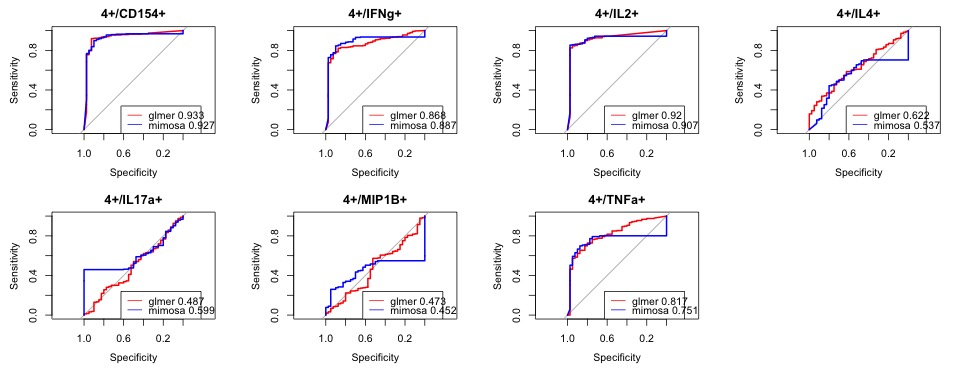
\includegraphics[width=12 cm]{figures/mimosaComparison} 
\caption{Comparison with MIMOSA (univariate COMPASS)}
\end{figure}
\end{frame}

%%%%%%%%%%%%%%%%%%%%%%%%%%%%%%%%%%%%%%%%%%%%%%%]

\begin{frame}
\frametitle{Subject-Response Model}
Performing analysis for each cell-subset at a time doesn't use all of the information available.
\pause
\vspace{0.3 cm} 
\begin{itemize}
\item Random Effects are correlated, can be estimated better simultaneously.
\vspace{0.3 cm}
\item Correlation structure might be of interest in itself. 
\pause
\vspace{0.3 cm}
\item Response is very likely not independent across cell-subsets.
\vspace{0.3 cm}
\item We might be able to improve classification of response by looking at several cell-subsets at once.  
\end{itemize}
\end{frame}

%%%%%%%%%%%%%%%%%%%%%%%%%%%%%%%%%%%%%%%%%%%%%%%]

\begin{frame}
\frametitle{A Hidden Markov Random Field Model}
\begin{framed}
Indexing: \textbf{i}-subject, \textbf{l}- stimulation, \textbf{j}- subset, \textbf{k}- cluster.
\end{framed}

Denote cluster (Response) by a $k \in \{0,1\}^{p}$ vector with $1$ indicating a responsive subset.
\pause
\vspace{0.3 cm}

We assume an Ising model for the dependence structure between subsets:
$$
P(k) \propto \sum_{j=1}^{p} k_{j} \theta_j + \sum_{s\neq t} k_{t} k_{s} \theta_{st},
$$$$
P(k_{j} = 1| k_{-j}) = \theta_{j} + \sum_{t\neq j } k_{t} \theta_{tj}.
$$

\pause
\vspace{0.3 cm}
We can induce sparsity through an $\ell_1$ penalty.

\end{frame}

%%%%%%%%%%%%%%%%%%%%%%%%%%%%%%%%%%%%%%%%%%%%%%%]

\begin{frame}
\frametitle{A Hidden Markov Random Field Model}
\begin{framed}
Indexing: \textbf{i}-subject, \textbf{l}- stimulation, \textbf{j}- subset, \textbf{k}- cluster.
\end{framed}

\vspace{0.3 cm}

$$
\nu_i \sim N_p(0, \Sigma),
$$$$
k_i \sim \text{Ising}(\theta),
$$$$
\text{logit}(\mu_{ijlk}) = X_{ijl} \beta + T_{ijl}\tau_{k_i} + \nu_{ij} ,
$$$$
y_{ijlk} \sim \text{Binom}(N_{il}, \mu_{ijlk}).
$$
\end{frame}

%%%%%%%%%%%%%%%%%%%%%%%%%%%%%%%%%%%%%%%%%%%%%%%]

\begin{frame}
\frametitle{HMRF Modle - Results}
\begin{figure}[]
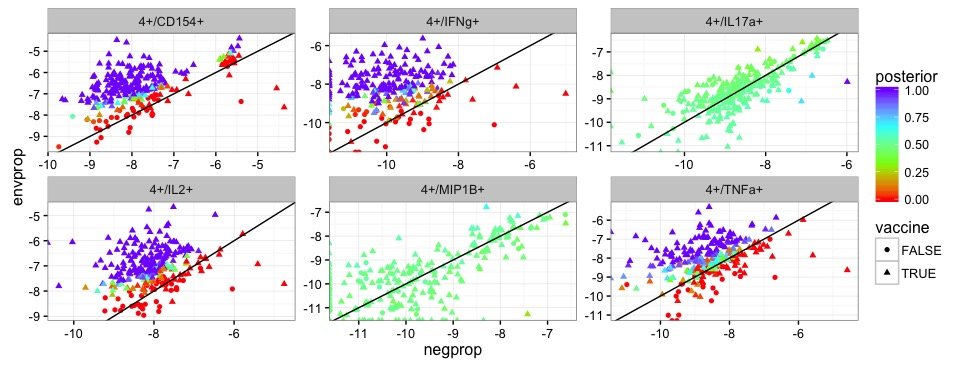
\includegraphics[width=12 cm]{figures/subsetBinomialScatter} \caption{Scatter Plot for HMRF Modle Model}
\end{figure}
\end{frame}
%%%%%%%%%%%%%%%%%%%%%%%%%%%%%%%%%%%%%%%%%%%%%%%]

\begin{frame}
\frametitle{Subset-Response Model - Results}
\begin{figure}[]
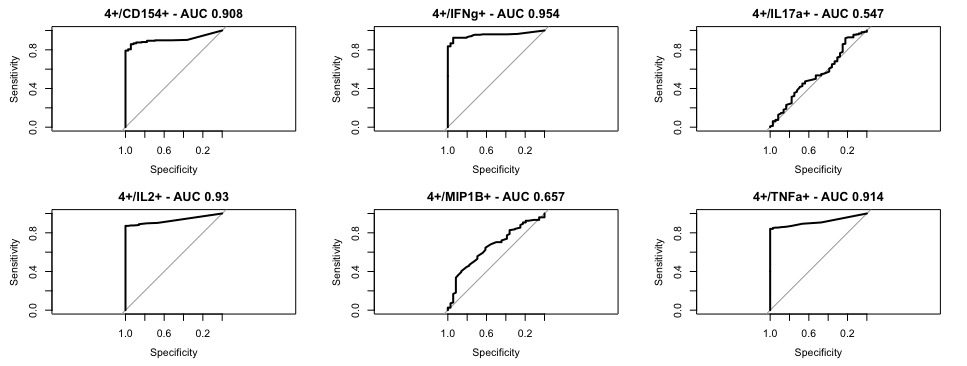
\includegraphics[width=12 cm]{figures/subsetBinomialAUC} \caption{ROC for HMRF Modle}
\end{figure}
\end{frame}

%%%%%%%%%%%%%%%%%%%%%%%%%%%%%%%%%%%%%%%%%%%%%%%]

\begin{frame}
\frametitle{Subset-Response Model - Results}
\begin{figure}[]
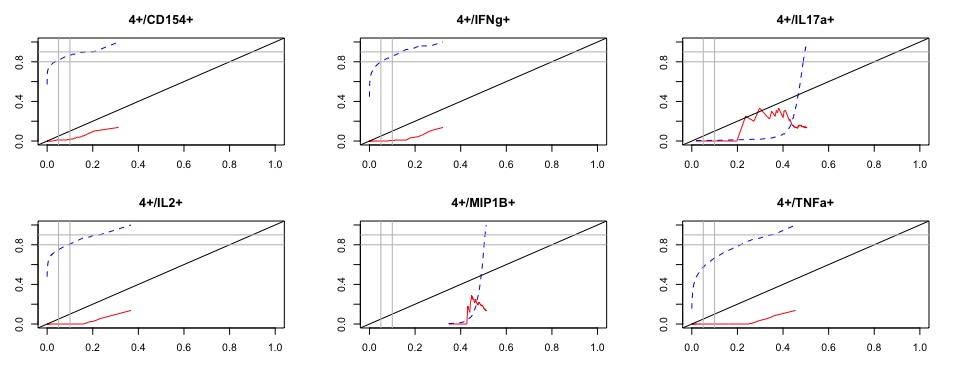
\includegraphics[width=12 cm]{figures/subsetBinomialFDR} \caption{FDR for HMRF Modle}
\end{figure}
\end{frame}

%%%%%%%%%%%%%%%%%%%%%%%%%%%%%%%%%%%%%%%%%%%%%%%]

\begin{frame}
\frametitle{Simulated Data Experiment}
\begin{itemize}
\item Posterior probabilities are not well calibrated.
	\begin{itemize}
	\item Might be due to true non-response.
	\end{itemize}
\pause
\vspace{0.5 cm}
\item Is the optimization algorithm estimating the model properly?
\vspace{0.5 cm}
\item Does the model fit the data well? 

\pause
\vspace{0.5 cm}
\item To find out:
	\begin{itemize}
	\item We generate data according to the estimated model.
	\item Fit should be perfect. 
	\item Is the artificial data similar to the real data?
	\end{itemize} 
\end{itemize}
\end{frame}

%%%%%%%%%%%%%%%%%%%%%%%%%%%%%%%%%%%%%%%%%%%%%%%]

\begin{frame}
\frametitle{Simulated Binomial Data - Results}
\begin{figure}[]
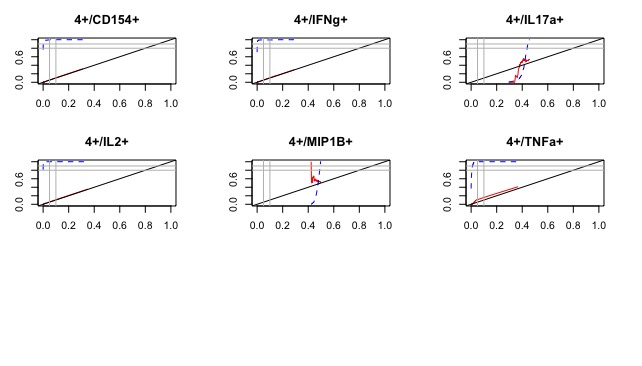
\includegraphics[width=12 cm]{figures/artificialBinomFDR} \caption{FDR for Simulated Binomial Data}
\end{figure}
\end{frame}

%%%%%%%%%%%%%%%%%%%%%%%%%%%%%%%%%%%%%%%%%%%%%%%]

\begin{frame}
\frametitle{Simulated Binomial Data - Results}
\begin{figure}[]
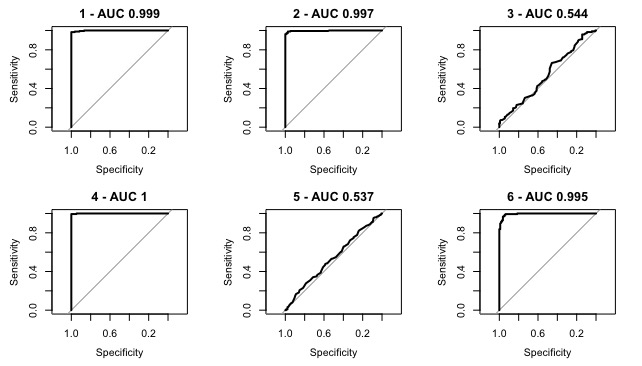
\includegraphics[width=12 cm]{figures/artificialBinomROC} \caption{ROC for Simulated Binomial Data}
\end{figure}
\end{frame}

%%%%%%%%%%%%%%%%%%%%%%%%%%%%%%%%%%%%%%%%%%%%%%%]

\begin{frame}
\frametitle{Simulated Binomial Data - Results}
\begin{figure}[]
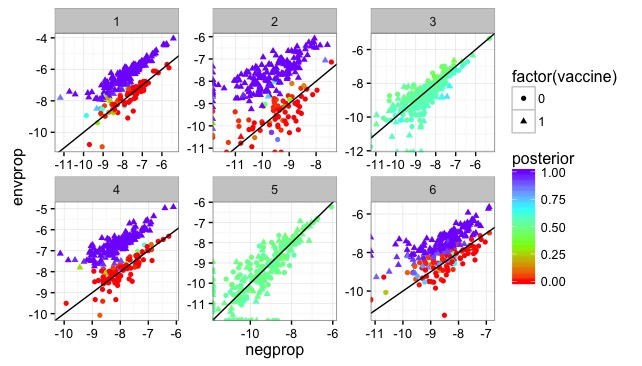
\includegraphics[width=12 cm]{figures/artificialBinomScatter} \caption{Scatter plot for Simulated Binomial Data}
\end{figure}
\end{frame}

%%%%%%%%%%%%%%%%%%%%%%%%%%%%%%%%%%%%%%%%%%%%%%%]

\begin{frame}
\frametitle{An Overdispersed Model}
We are clearly missing some variablility... 
\vspace{0.3 cm}

Assume a Beta-Binomial Model:
$$
\text{logit}(\mu) = X\beta + T\tau + \nu,
$$$$
p \sim \text{Beta}(M\mu, M(1-\mu)), \;\;\;\;\; M>0,
$$$$
y \sim \text{Binom}(N, p).
$$
\end{frame}

%%%%%%%%%%%%%%%%%%%%%%%%%%%%%%%%%%%%%%%%%%%%%%%]

\begin{frame}
\frametitle{An Overdispersed Model - Recap}
\begin{framed}
Indexing: \textbf{i}-subject, \textbf{l}- stimulation, \textbf{j}- subset, \textbf{k}- cluster.
\end{framed}

$$
\nu_i \sim N(0, \Sigma),
$$$$
k_i \sim \text{Ising}(\theta).
$$$$
\text{logit}(\mu_{ijlk}) = X_{ijl} \beta + T_{ijl}\tau_{k_i} + \nu_{ij} ,
$$$$
y_{ijlk} \sim \text{Beta-Binomial}(N_{il}, \mu_{ijlk}, M_j) ,
$$
\end{frame}

%%%%%%%%%%%%%%%%%%%%%%%%%%%%%%%%%%%%%%%%%%%%%%%]

\begin{frame}
\frametitle{How close are we to the distribution of the data?}
\begin{figure}[]
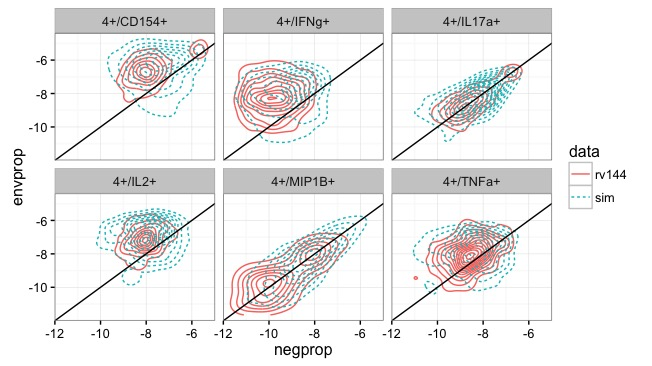
\includegraphics[width=12 cm]{figures/simVsRealContour} 
\end{figure}
\end{frame}

%%%%%%%%%%%%%%%%%%%%%%%%%%%%%%%%%%%%%%%%%%%%%%%]

\begin{frame}
\frametitle{Overdispersed Model - Results}
\begin{figure}[]
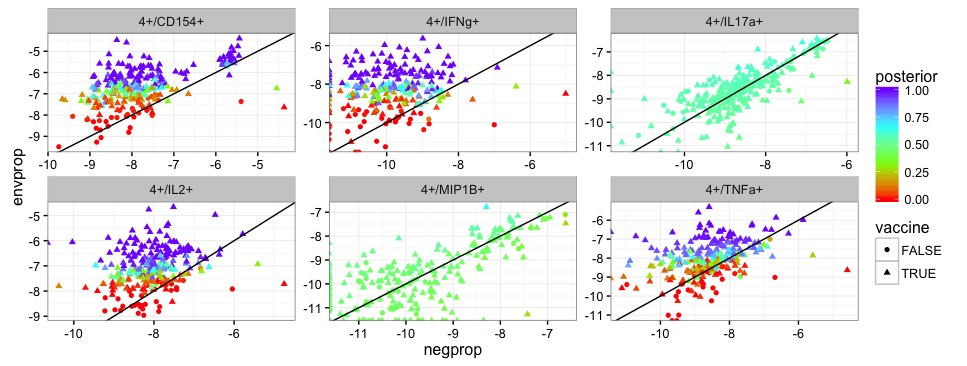
\includegraphics[width=12 cm]{figures/marginalBBscatter} \caption{Scatter plot for Overdispersed Model }
\end{figure}
\end{frame}

%%%%%%%%%%%%%%%%%%%%%%%%%%%%%%%%%%%%%%%%%%%%%%%]

\begin{frame}
\frametitle{Overdispersed Model - Results}
\begin{figure}[]
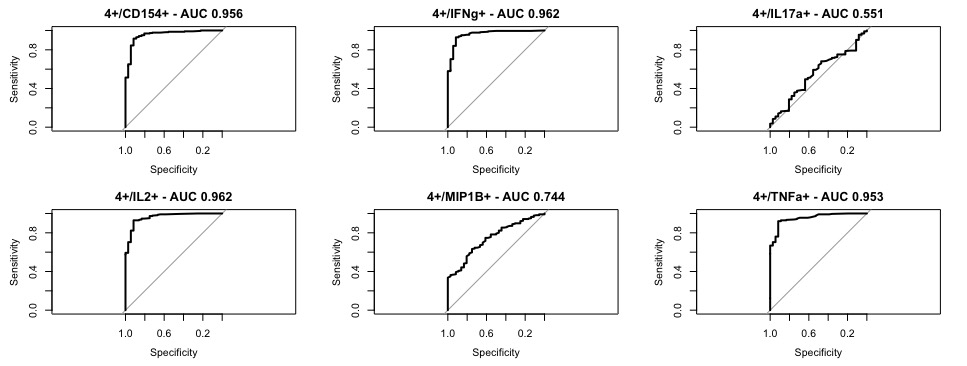
\includegraphics[width=12 cm]{figures/marginalBBroc} \caption{ROC for Overdispersed Model}
\end{figure}
\end{frame}

%%%%%%%%%%%%%%%%%%%%%%%%%%%%%%%%%%%%%%%%%%%%%%%]

\begin{frame}
\frametitle{Overdispersed Model - Results}
\begin{figure}[]
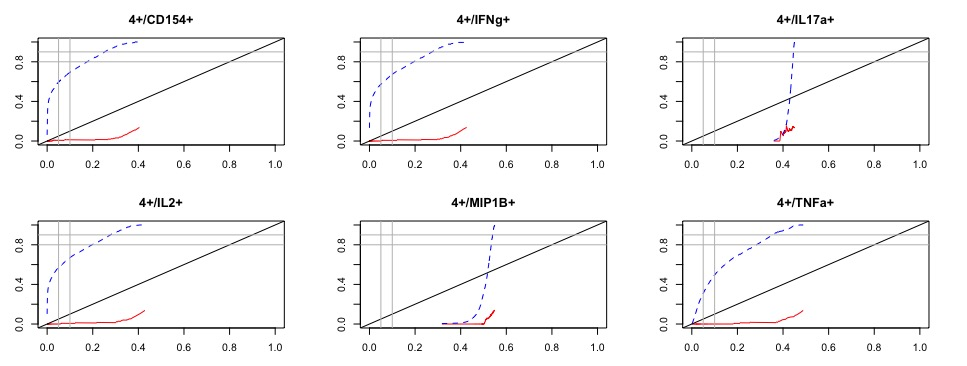
\includegraphics[width=12 cm]{figures/marginalBBfdr} \caption{FDR for Overdispersed Model}
\end{figure}
\end{frame}

%%%%%%%%%%%%%%%%%%%%%%%%%%%%%%%%%%%%%%%%%%%%%%%]

\begin{frame}
\frametitle{RV144 - Booleans Dataset}
226 vaccinees, and 36 placebos, 24 cell-subsets.
\begin{figure}[]
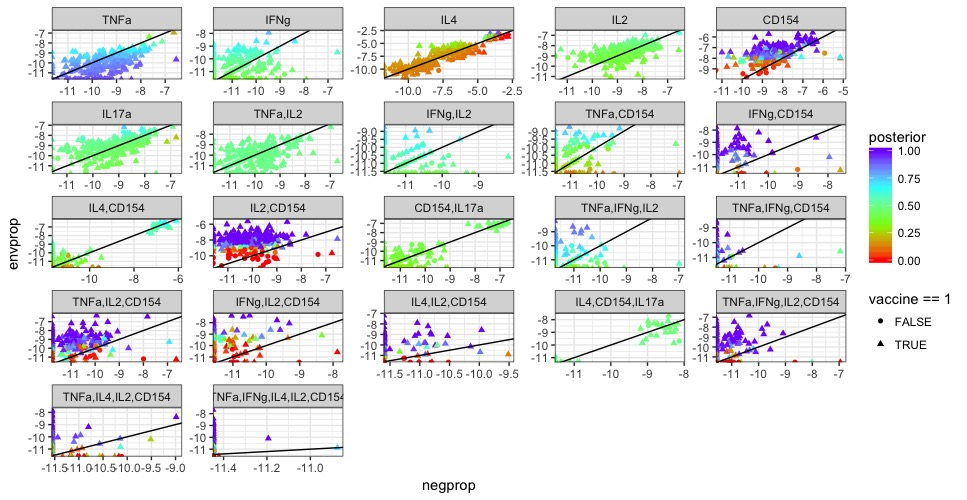
\includegraphics[width=13.2 cm]{figures/booleansFullScatter}
\end{figure}
\end{frame}

%%%%%%%%%%%%%%%%%%%%%%%%%%%%%%%%%%%%%%%%%%%%%%%]

\begin{frame}
\frametitle{RV144 - Booleans Dataset}
\begin{figure}[]
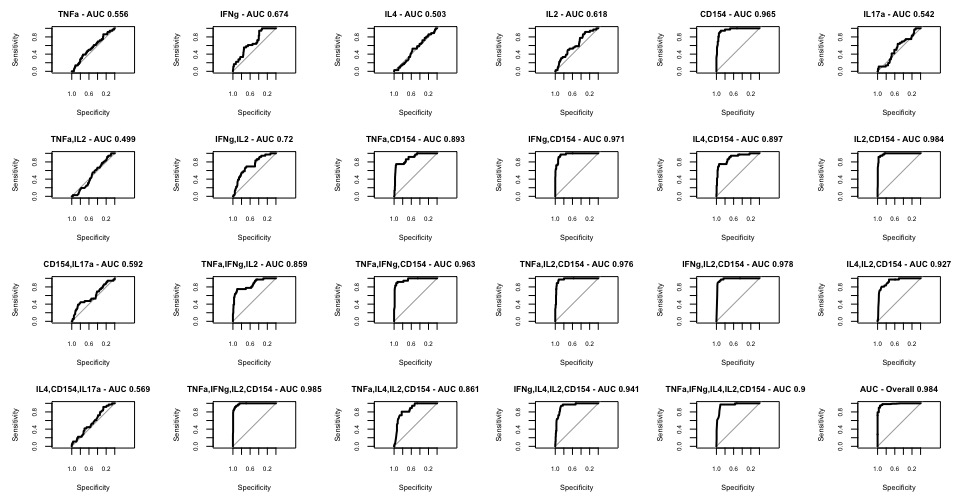
\includegraphics[width=12 cm]{figures/booleansAUC2} \caption{ROC for RV144 booleans dataset}
\end{figure}
\end{frame}

%%%%%%%%%%%%%%%%%%%%%%%%%%%%%%%%%%%%%%%%%%%%%%%]

\begin{frame}
\frametitle{RV144 - Booleans Dataset}
\begin{figure}[]
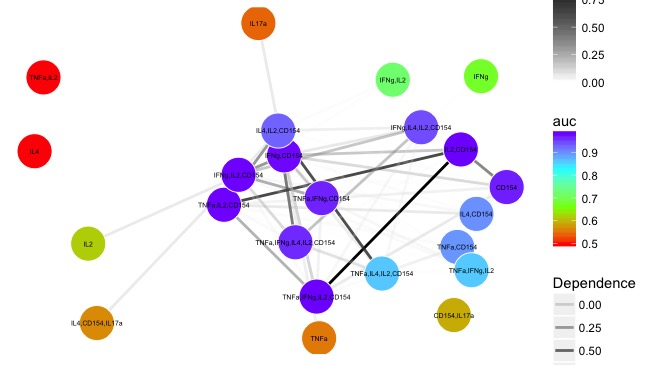
\includegraphics[width=10 cm]{figures/booleansGraphAUC} \caption{Estimated Ising Model}
\end{figure}
\end{frame}

%%%%%%%%%%%%%%%%%%%%%%%%%%%%%%%%%%%%%%%%%%%%%%%]

\begin{frame}
\frametitle{RV144 - Booleans Dataset}
\begin{figure}[]
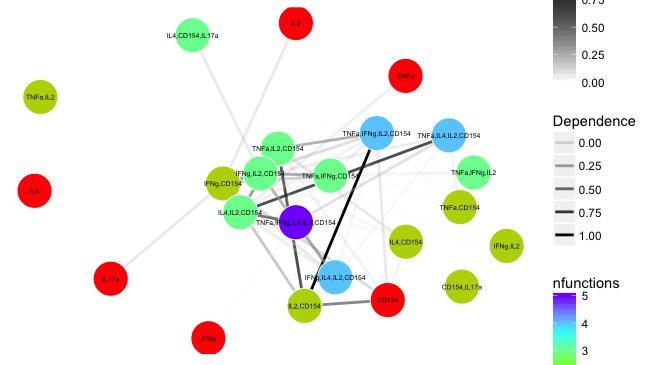
\includegraphics[width=10 cm]{figures/booleansGraphFunctions} \caption{Estimated Ising Model}
\end{figure}
\end{frame}

%%%%%%%%%%%%%%%%%%%%%%%%%%%%%%%%%%%%%%%%%%%%%%%]

\begin{frame}
\frametitle{Controlled Human Malaria Infection Study}
\begin{itemize}
\item 9 Tanzanian adults were infected with Malaria.
	\begin{itemize}
	\item +3 controls.
	\end{itemize}
	\vspace{0.75 cm}
	
\item Blood samples were collected at 6 time points.
	\begin{itemize}
	\item Day 0, day 9, blood  parasitemia, Day 28, Day 56, Day 168.
	\end{itemize}
	\vspace{0.75 cm}

\item Two types of stimulation:
	\begin{itemize}
	\item Infected/uninfected blood-cells.
	\end{itemize}
	\vspace{0.75 cm}
	
\item 113 measured cell-types divided into 8 groups. 
\end{itemize}
\end{frame}

%%%%%%%%%%%%%%%%%%%%%%%%%%%%%%%%%%%%%%%%%%%%%%%]

\begin{frame}
\frametitle{Controlled Human Malaria Infection Study}
\begin{figure}[]
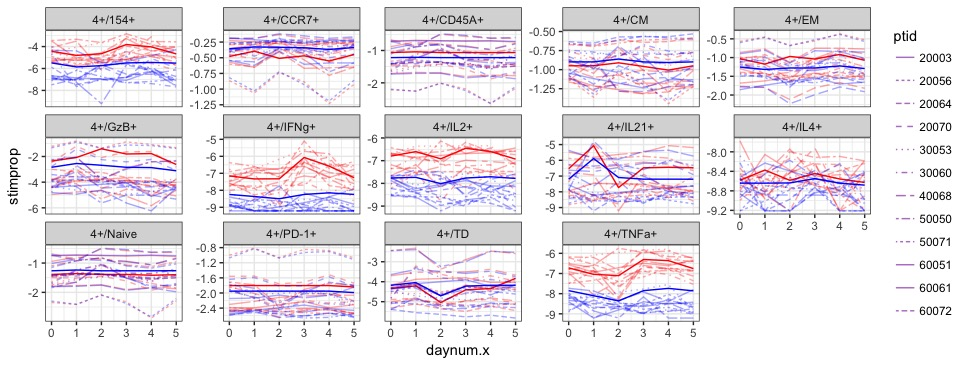
\includegraphics[width=13 cm]{figures/4plusSmoothed} \caption{Stimulated vs. Unstimulated}
\end{figure}
\end{frame}

%%%%%%%%%%%%%%%%%%%%%%%%%%%%%%%%%%%%%%%%%%%%%%%]

\begin{frame}
\frametitle{Controlled Human Malaria Infection Study}
\begin{figure}[]
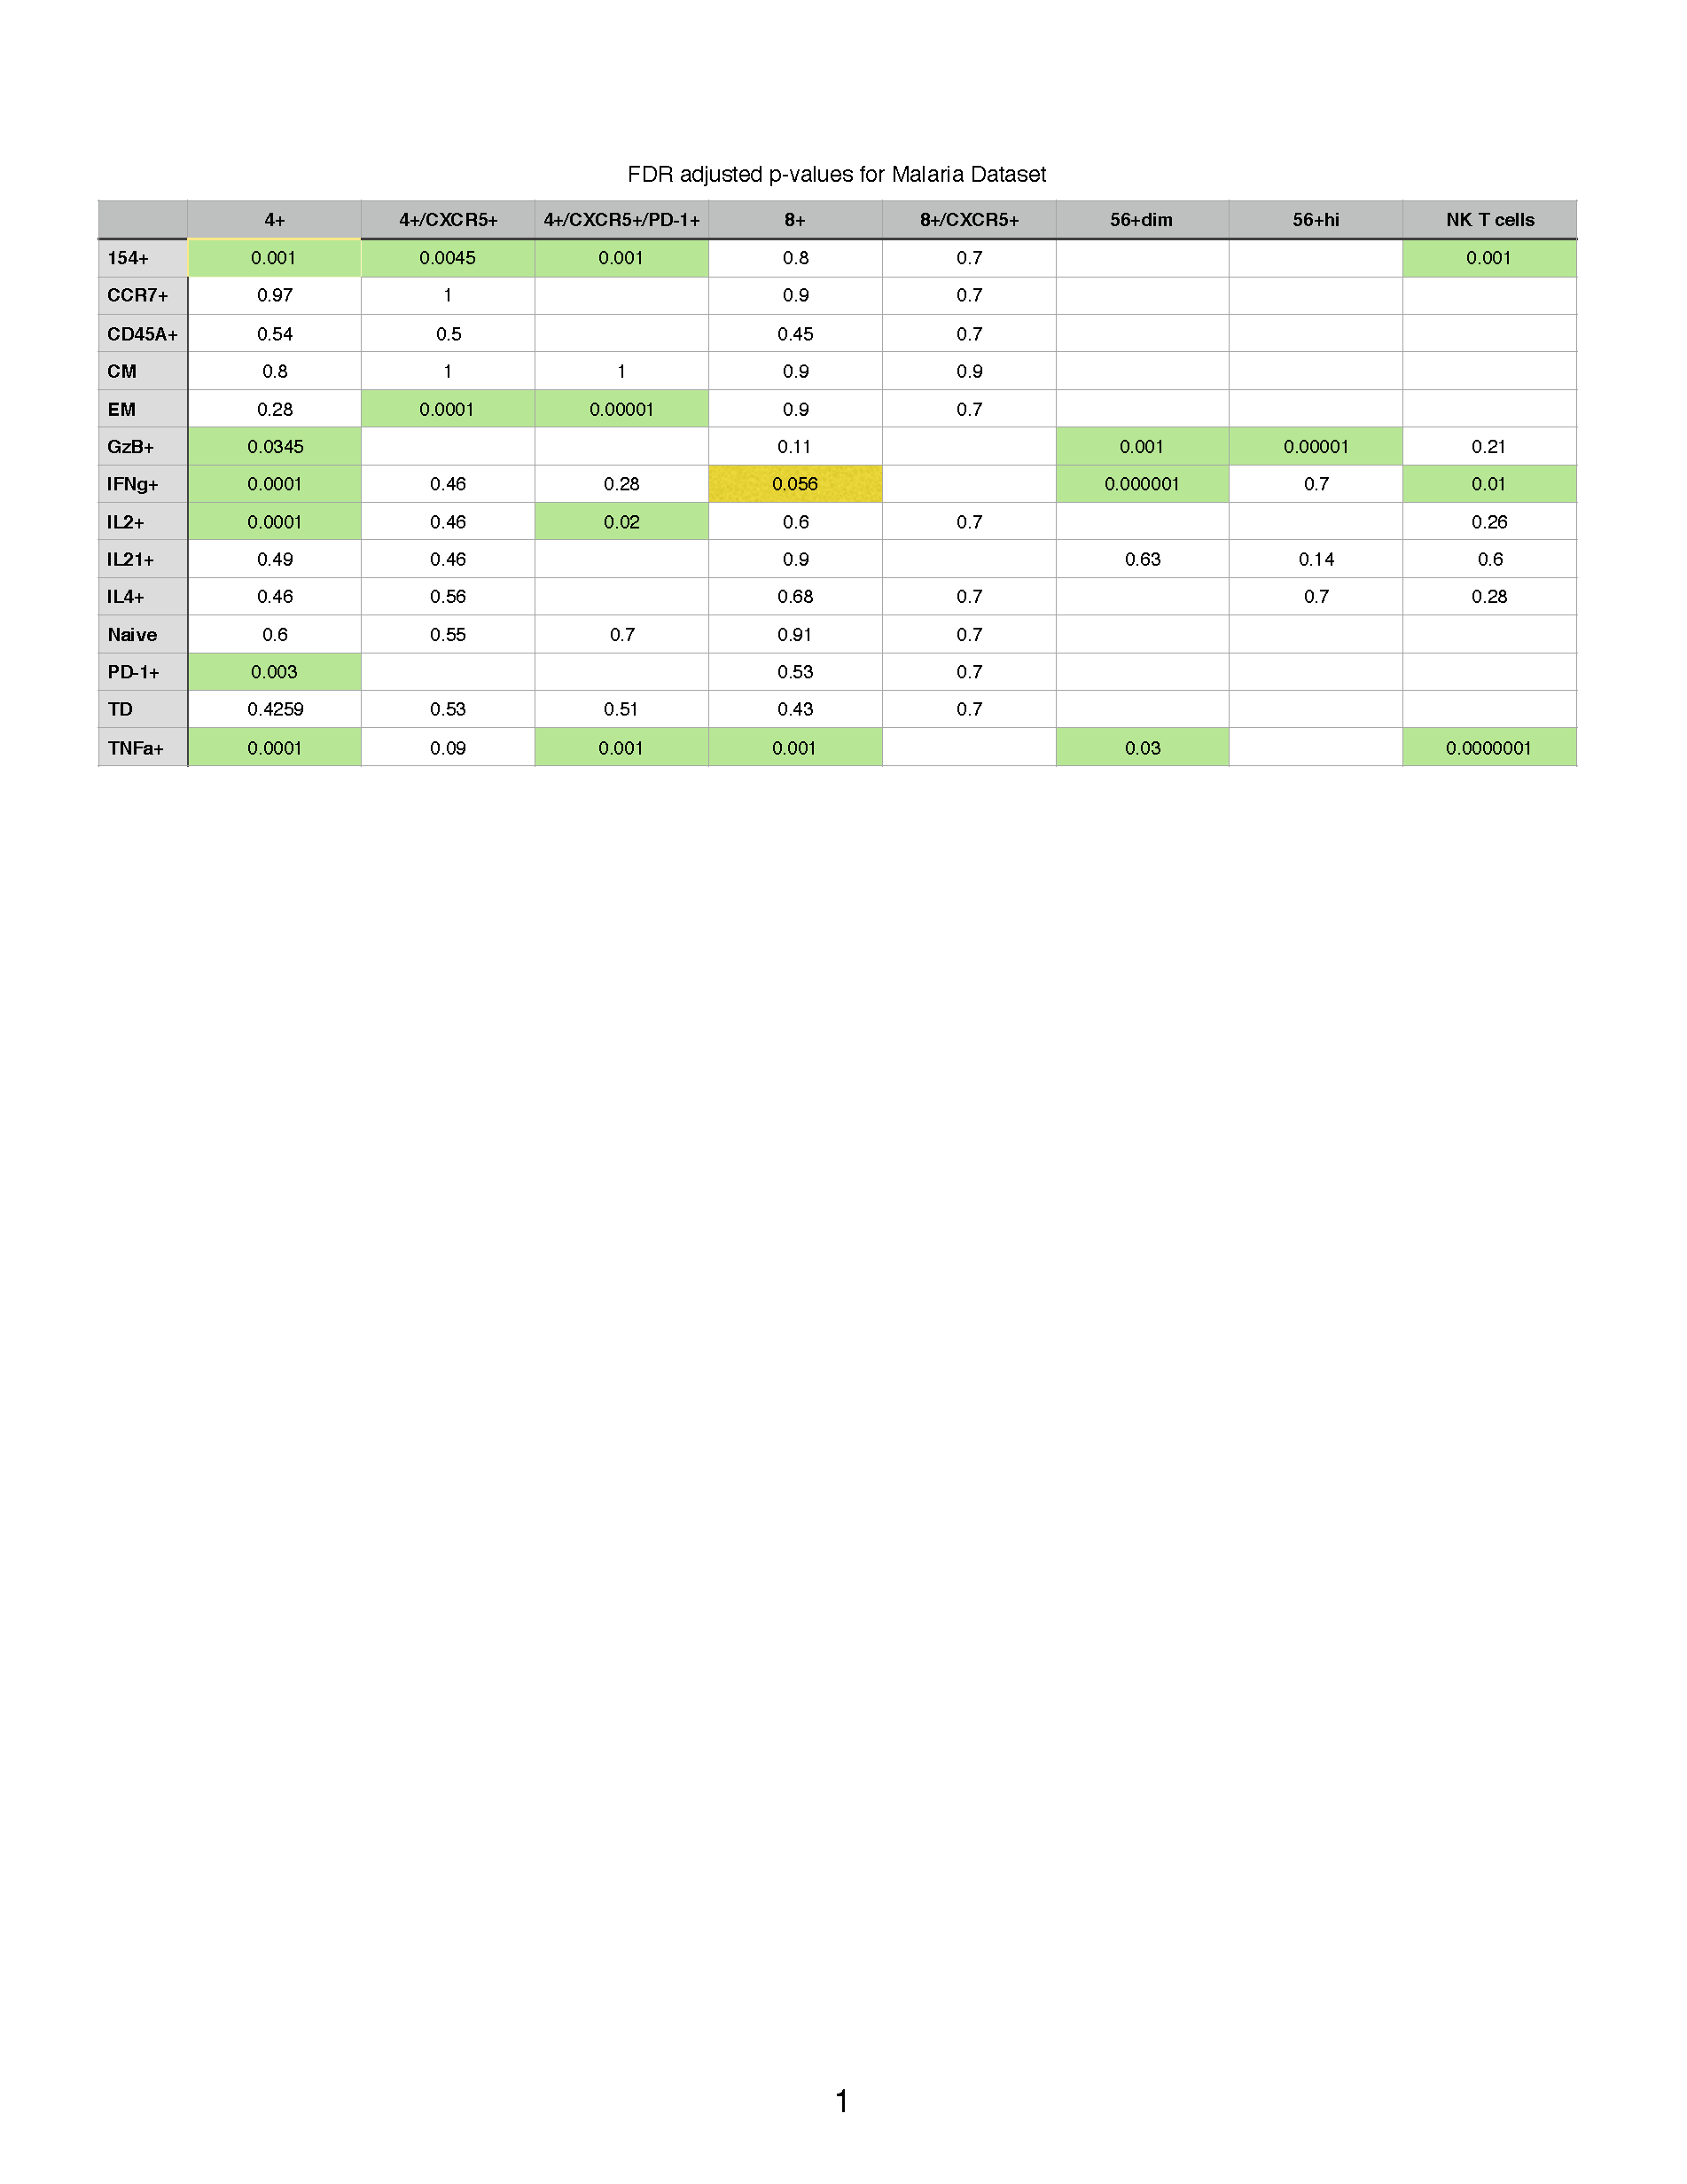
\includegraphics[width=12 cm]{figures/malariaQvals} \caption{Stimulated vs. Unstimulated}
\end{figure}
\end{frame}

%%%%%%%%%%%%%%%%%%%%%%%%%%%%%%%%%%%%%%%%%%%%%%%]

\begin{frame}
\frametitle{Controlled Human Malaria Infection Study}
\begin{figure}[]
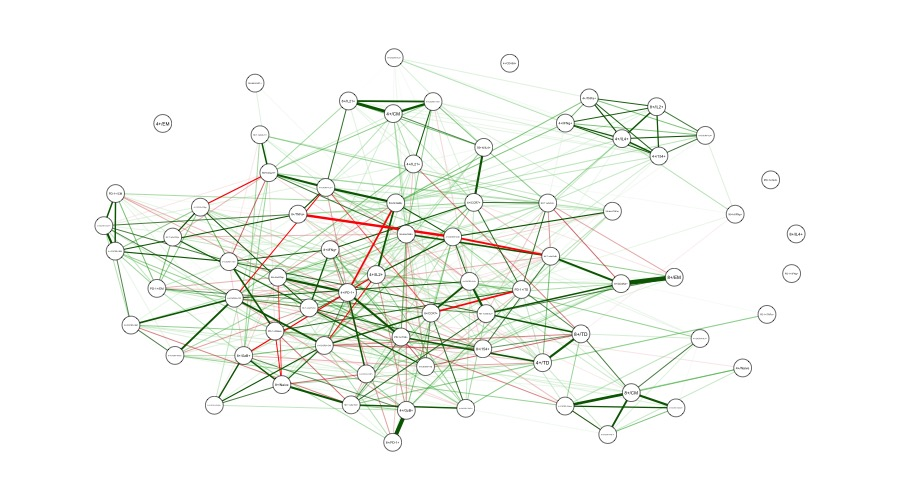
\includegraphics[width=12 cm]{figures/malariaGraph} \caption{Stimulated vs. Unstimulated}
\end{figure}
\end{frame}

%%%%%%%%%%%%%%%%%%%%%%%%%%%%%%%%%%%%%%%%%%%%%%%]

\begin{frame}
\frametitle{Computation}

\end{frame}

%%%%%%%%%%%%%%%%%%%%%%%%%%%%%%%%%%%%%%%%%%%%%%%]

\begin{frame}
\begin{center}
\huge{Thank you!}

\vspace{2 cm}
\LARGE{Questions?}

\vspace{1cm}
\large{AmitMeir@uw.edu}
\end{center}
\end{frame}


\end{document}
